 \hypertarget{index_intro_sec}{}\subsection{Introduction}\label{index_intro_sec}
This project is about using an W\+S2811 or W\+S2812 lightstribe with an A\+V\+R controller. It is possible to handle up to 250 L\+E\+Ds at the same time, so I chose an Atmega328p with enough R\+A\+M amount. If you want to handle less L\+E\+Ds you can use most parts of this project with every A\+V\+R. The A\+V\+R is programmed to receive the light data over U\+A\+R\+T so you can control the L\+E\+Ds by using a serial interface. The interface uses a specified simple protocol which is described in \hyperlink{index_protocol_sec}{protocol overview} section. Everything has been developed in a university course to control the lights of a Christmas tree. In the original implementation there were some further components included. This is a simplified version of the implementation so that everyone can use it. As an example for controlling the L\+E\+Ds using a smart phone the \hyperlink{index_esp_sec}{control via E\+S\+P8266} section shows how this could be done by using a webserver on the E\+S\+P8266. You can use everything else that provide a serial interface (maybe connect with a bluetooth serial module). The structure of this documentation is split in a hardware part for the A\+V\+R that describes the basic hardware that should be used. The next part is about how the software is working on the A\+V\+R that handles the L\+E\+Ds and different effects. You may include some more stuff in your own. After that you can see a small protocol overview, where you find which command can be sent to the A\+V\+R to control the L\+E\+Ds. Be aware that at the initialization state all L\+E\+Ds are off. At the last point you can find an example how to use the implementation with an E\+S\+P8266 with a webserver. You will find the source code for the E\+S\+P8266 and the basic hardware setup.\hypertarget{index_hardware_sec}{}\subsection{Hardware}\label{index_hardware_sec}
The basic hardware you need is a A\+V\+R controller an some W\+S2811 or W\+S2812 L\+E\+Ds you want to control. The A\+V\+R controller should have an hardware U\+A\+R\+T, otherwise you need to write some code for a software serial. In the project we chose an Atmega328p that has enough R\+A\+M to control 250 L\+E\+Ds. The internal software structure buffers the color data for the L\+E\+Ds to achieve an accurate timing, see section \hyperlink{index_software_sec}{software implementation}. The A\+V\+R can be used with the internal clock at 8 M\+Hz, remember to clear the clock divider fuse. Otherwise an external 8 M\+Hz or 16 M\+Hz clock source can be used, the definition \hyperlink{globals_8h_a43bafb28b29491ec7f871319b5a3b2f8}{F\+\_\+\+C\+P\+U} must be set to the frequency you chose (remember to set the fuses for an external clock source). As an example the figure \hyperlink{index_one}{one} shows using an external 16 M\+Hz crystal. \label{index_one}%
\hypertarget{index_one}{}%

\begin{DoxyImage}
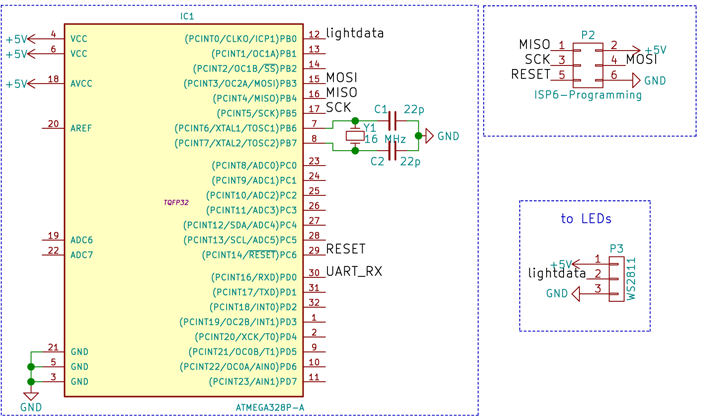
\includegraphics[width=\textwidth,height=\textheight/2,keepaspectratio=true]{Ws2811_Atmega328_schematic.png}
\caption{schematic of the A\+V\+R to controll W\+S2812/\+W\+S2811}
\end{DoxyImage}
 As you can see in the picture the A\+V\+R is programmed by using the I\+S\+P interface. The W\+S2812/\+W\+S2811 get the same voltage as the A\+V\+R, the light data is available at Pin\+B0, you may change this if you like. Referring to the L\+E\+Ds be aware of the current amount they may draw if every L\+E\+D has its full brightness. One W\+S2812 can draw up to 60 m\+A, so one meter with 30 L\+E\+Ds already need 1,8 A. If you want to control more L\+E\+Ds you may have a problem with the voltage drop along the stribe. For example if you control 180 L\+E\+Ds at six meters you not only need 10,8 A, furthermore you will probably have a voltage drop up to 2 V. To reduce the voltage drop you must increase the wire size with parallel wires to you stribe. You can see the voltage drop if you set all L\+E\+Ds to white. If you have only a small voltage drop every L\+E\+D will have the same color. If the voltage drop is too much you can see that the last L\+E\+Ds will have less blue color, so they will light in a warm white color even up to red. If you want to try out the L\+E\+Ds with the A\+V\+R you can build up everything on a breadboard. Pinheaders can be soldered easy at the light stribes as you can see in the figure \hyperlink{index_two}{two}. \label{index_two}%
\hypertarget{index_two}{}%

\begin{DoxyImage}
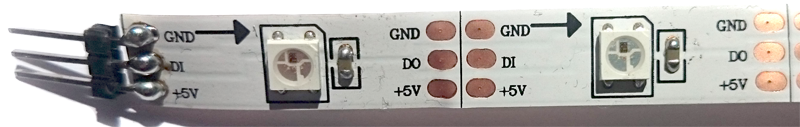
\includegraphics[width=\textwidth,height=\textheight/2,keepaspectratio=true]{WS2812.png}
\caption{W\+S2812 stribe with pin header}
\end{DoxyImage}
The connect G\+N\+D to the common ground with the A\+V\+R, 5 V should be connected to a power supply that can handle the current you need. D\+I is the data in line, this should be connected to Pin\+B0 at the A\+V\+R. The stribe is like a big shifting register, all the data you sent is shifted bit by bit through the stribe. So D\+O is the data out pin, you see some data at this pin if all L\+E\+Ds before had already received their color data. The one wire protocol of the L\+E\+Ds is described in the \hyperlink{index_software_sec}{software implementation} section.\hypertarget{index_software_sec}{}\subsection{software implementation}\label{index_software_sec}
\hypertarget{index_install_sec}{}\subsection{Installation}\label{index_install_sec}
\hypertarget{index_step1}{}\subsubsection{Step 1\+: Opening the box}\label{index_step1}
etc...\hypertarget{index_protocol_sec}{}\subsection{protocol overview}\label{index_protocol_sec}
\hypertarget{index_esp_sec}{}\subsection{control via E\+S\+P8266}\label{index_esp_sec}
author\+: Florian Wank, 2016 